\section{Section}
\pagenumbering{arabic}
\setcounter{page}{1}

Einen guten Forscher erkennt man daran, dass er alle Hintergruende erforscht.
Ich, Prof. Lactosius, bin natuerlich ein guter Forscher. Deshalb habe ich auch
die Quelle der Schulmilch, die Kuehe, gruendlich erforscht.

\subsection{Subsection}

Ich weiss schon, was ihr jetzt sagen werdet. Jeder weiss, wie eine Kuh aussieht.
Aber auch bei den Kuehen habe ich kleine und groessere Unterschiede entdeckt.
Also los, folgt mir ins Land der Kuehe. 

\begin{figure}[h]
   \begin{center}
   \caption{Example Figure}\label{fig:example-figure}\smallskip
   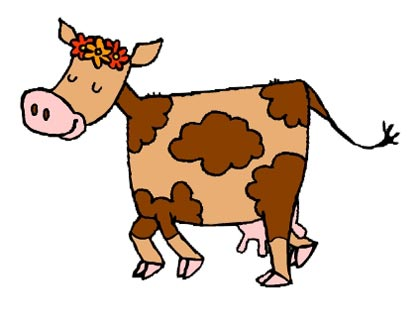
\includegraphics[clip=true]{test-image}
\end{center}
\end{figure}

\minisec{Minisec}

...



